% vim:ft=tex:
%

\documentclass[12pt]{article}

\author{Arthur Oliveira de Rosso}
\title{GoBov - Sistema Web de Gerenciamento Bovino.}

\usepackage{times}
\usepackage[utf8]{inputenc}
\usepackage[T1]{fontenc}
\usepackage[alf]{abntex2cite}
\usepackage[brazil]{babel}
\usepackage[normalem]{ulem}
\usepackage{indentfirst}
\usepackage[top=3cm,left=3cm,bottom=2cm,right=2cm]{geometry}
\useunder{\uline}{\ul}{}
\usepackage{graphicx}
\graphicspath{{img/}}

\newenvironment{citar}{\begin{changemargin}{4cm}{0cm}\fontsize{10pt}{12pt}\selectfont}{\end{changemargin}}

\begin{document}



\makeatletter
\begin{titlepage}
	\begin{center}

		INSTITUTO FEDERAL DE EDUCAÇÃO, CIÊNCIA E TECNOLOGIA 

		DO RIO GRANDE DO SUL

		CAMPUS CANOAS

		CURSO TÉCNICO EM INFORMÁTICA INTEGRADO AO ENSINO MÉDIO

		\vfill
		\vfill

		\@author

		\vfill

		\textbf{\@title}

		\vfill

		\textbf{Orientador:} Rodrigo Noll

		\vfill

		Canoas, \today

	\end{center}
\end{titlepage}
\newpage


\section{Proposta de Trabalho de Conclusão de Curso}

\subsection{Descrição do Problema}
Uma análise do processo de criação de bovinos em uma propriedade rural, demonstra que o ciclo de vida do animal necessita de um acompanhamento rigoroso e contínuo. Os registros de informações relativas aos animais adquirem profunda relevância uma vez que a falta de informações pode ocasionar um descontrole sanitário.

Segundo \citeonline{Marcelino16}, na bovinocultura brasileira, seja ela de corte ou de leite, devemos nos atentar para todos os fatores que possam prejudicar ou diminuir a produção do animal, como por exemplo, as doenças. Muitas  delas podem ser evitadas se os animais forem vacinados, por isso é importante que o produtor esteja sempre atento aos programas de vacinação adotados em cada região, levando em consideração a maneira mais adequada para tratar os animais, pois há vacinas que são aplicadas no rebanho todo, outras são aplicadas somente em certas categorias de animais, selecionando idade e até mesmo o sexo.

A problemática dos pecuaristas, que são o público alvo do presente trabalho, se dá no fato de que embora o registro individual dos animais seja fundamental por conter informações indispensáveis ao manejo do animal, não é essa uma prática habitual por se tratar de uma tarefa muitas vezes complicada, quando feita somente no papel, pois este registro pode ser perdido ou danificado.

\subsection{Proposta de solução}

Um sistema web de gerenciamento bovino, o qual possibilita ao usuário registrar seus animais de modo a otimizar o tempo gasto no registro do tratamento através de um controle de peso e remédios.

\subsection{Objetivos}

\subsubsection{Objetivo Geral}

Implementar um sistema web que visa gerenciar os animais de uma propriedade proporcionando um controle sanitário afim de possibilitar a identificação de possíveis focos de doenças e epidemias, bem como a aplicação de um controle de peso capaz de identificar os ganhos obtidos.

\subsubsection{Objetivos Específicos}

\begin{itemize}
	\item Escolher as tecnologias a serem utilizadas no sistema;
	\item Pesquisar as necessidades dos pecuaristas e de que maneira o sistema pode auxiliá-los;
	\item Modelar o sistema;
	\item Identificar as informações relevantes sobre o ciclo de vida do animal bovino;
	\item Realizar pesquisas de sistemas relacionados para identificar pontos onde há um nicho de mercado inexplorado;
	\item Implementar o sistema.
	\item Realizar testes do sistema.
	\item Avaliar o sistema na realidade dos pecuaristas.
\end{itemize}

\section{Trabalhos Relacionados}

% TODO: Nesse capitulo deve aparecer a analise que foi realizada em aplicativos, aplicações, sistemas, plataformas, sites, etc., que guardam semelhança com a proposta a ser desenvolvida no projeto.

Durante o levantamento de dados foram buscadas plataformas que trabalham de forma semelhante ao presente sistema, como por exemplo o BovControl, o JetBov e o A3Pecuária.

\subsection{BovControl}

BovControl é uma ferramenta de coleta e análise de dados provenientes da pecuária para melhorar a performance da produção de carne, leite ou genética \cite{bovcontrol10}. 

É disponibilizado em forma de aplicativo e possui um plano gratuito, no qual é possível gerir um rebanho e faz os seguintes manejos nos animais: saída, lote, exame de toque, controle reprodutivo, idade da cria, idade do desmame, medicamento, origem, pesagem, perímetro escrotal, leite, teste diagnóstico, tipo de entrada, vacina, vermifugação. Também é possível visualizar seus dados em um dashboard na internet.

Possui uma parte de relatórios com apenas 2 gráficos, um do total de animais e do tipo de produção do animal(como leite, engorda e genética), e outro do total de animais e do gênero(macho ou fêmea). 

Possui 3 planos profissionais que variam de R\$ 22,99 a R\$ 32,99 por mês. Estes planos incluem gestor financeiro, gestor de tarefas, multiusuários, relatórios personalizados, importação de animais por planilha e estoque de maquinário.  

A seguir, uma imagem mostrando a página inicial do sistema BovControl versão web.

\begin{figure}[!h]
	\begin{center}
		\caption{Dashboard do BovControl}
		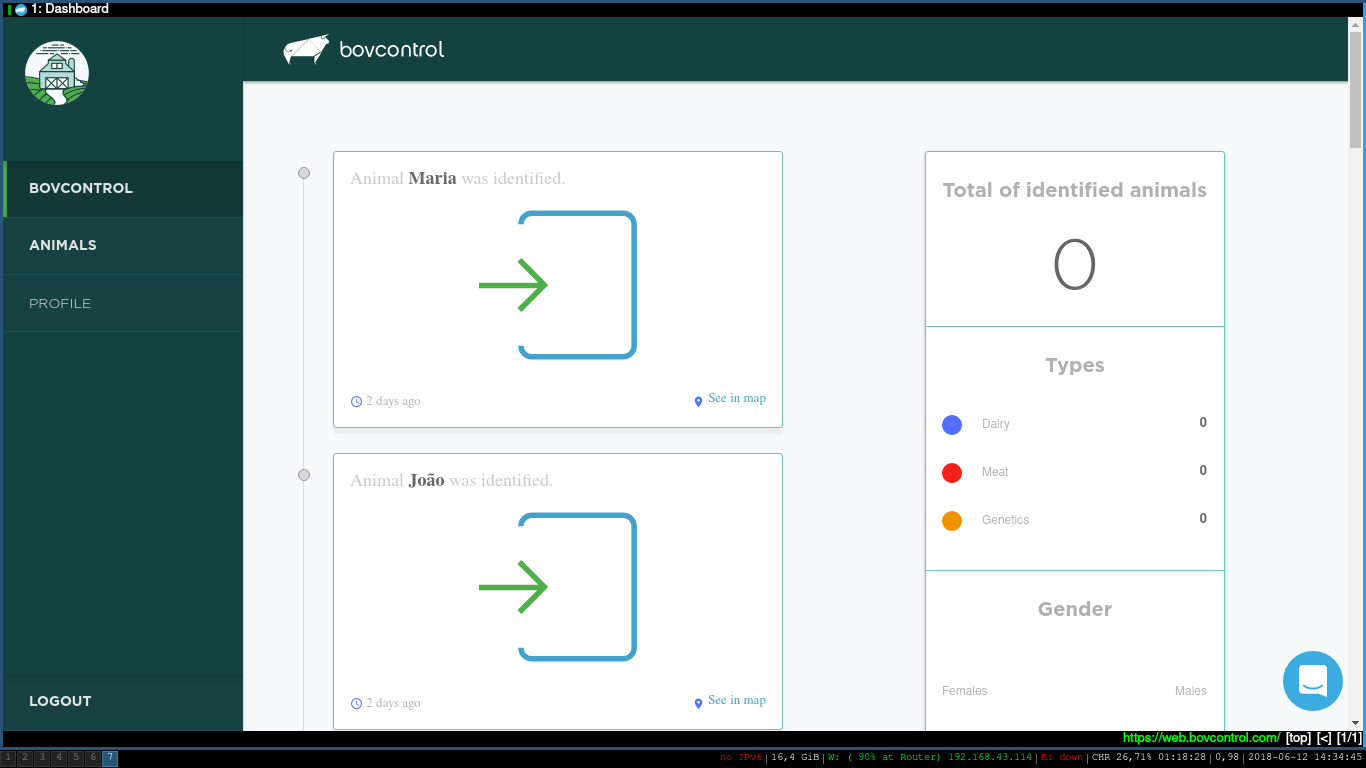
\includegraphics[width=6in]{img/bovcontrol.png}

		\floatfoot{Fonte: Autoria própria.}
	\end{center}
\end{figure}


%\begin{figure}[!h]
%\begin{center}
%\caption{BovControl versão mobile - Página inicial}
%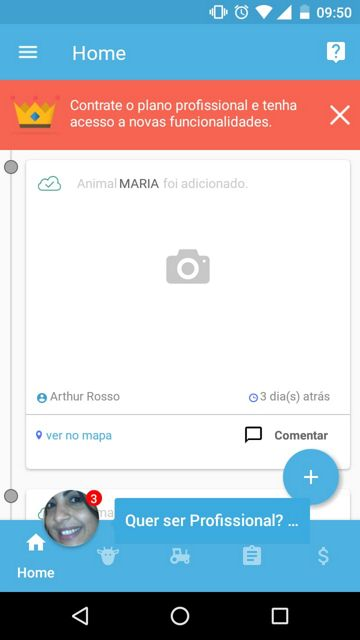
\includegraphics[width=6in]{img/bovcontrolapp1.jpg}

%\floatfoot{Fonte: Autoria própria.}
%\end{center}
%\end{figure}

%\begin{figure}[!h]
%\begin{center}
%\caption{BovControl versão mobile - Opções de ações}
%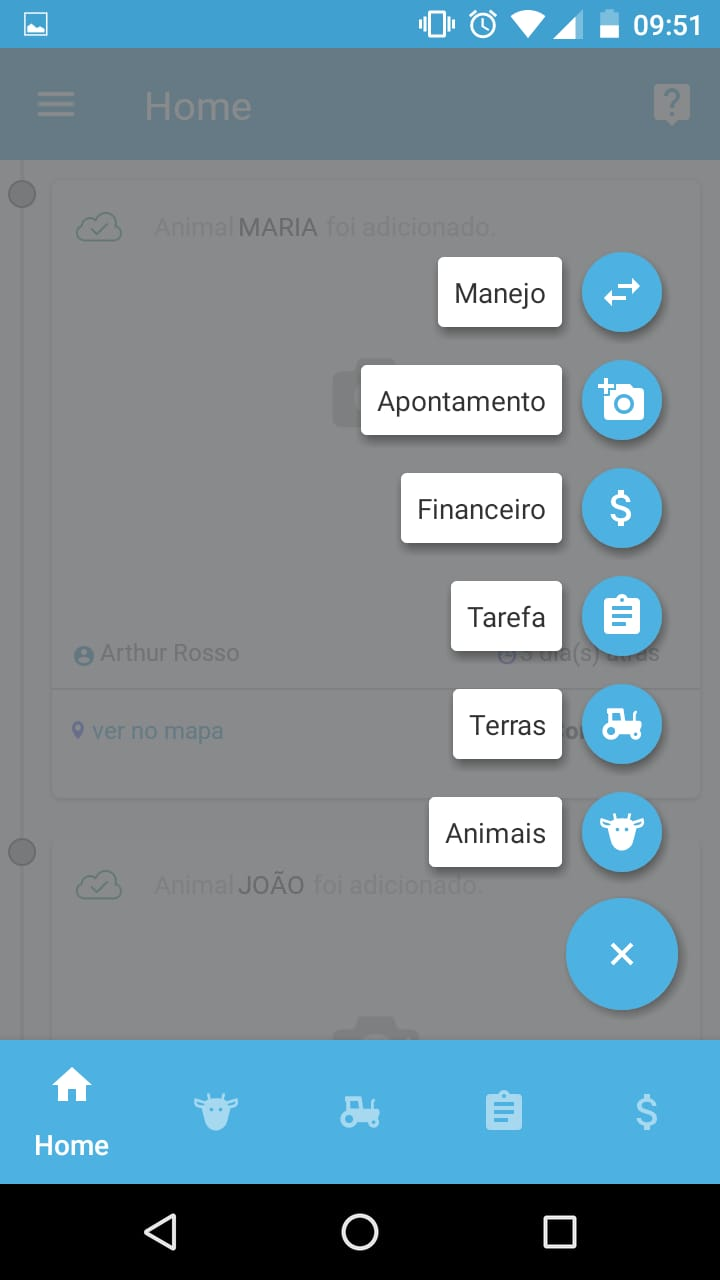
\includegraphics[width=6in]{img/bovcontrolapp2.jpeg}

%\floatfoot{Fonte: Autoria própria.}
%\end{center}
%\end{figure}

\newpage


\subsection{JetBov}

Segundo \citeonline{jetbov16}, esse é um sistema que tem como objetivo a gestão da fazenda, da cria até a terminação, a pasto, no semi-confinamento ou confinamento, com um controle de custos com o propósito de aumento da rentabilidade. 

Não possui versão gratuita, porém tem uma versão de testes por 21 dias, após isso é necessário realizar um orçamento individual.

O sistema apresenta 2 versões, uma web e outra mobile, a mobile é simples contendo apenas uma página com animais e um botão contendo as opções de manejo como adicionar um novo animal e sua identificação, registros sanitários como vacinações, medicações, exames, vermifugações, etc, adicionar a morte de um animal, o desmame, o parto e pesagem.

A versão web é mais completa contendo um painel de dados da fazenda, com gráficos de animais por sexo, animais por lote, peso por lote e algumas informações como número total de animais da fazenda, peso total da fazenda. 

A seguir, uma imagem mostrando a página inicial do sistema JetBov versão web.

\begin{figure}[!h]
	\begin{center}
		\caption{Página inicial da versão web do JetBov}
		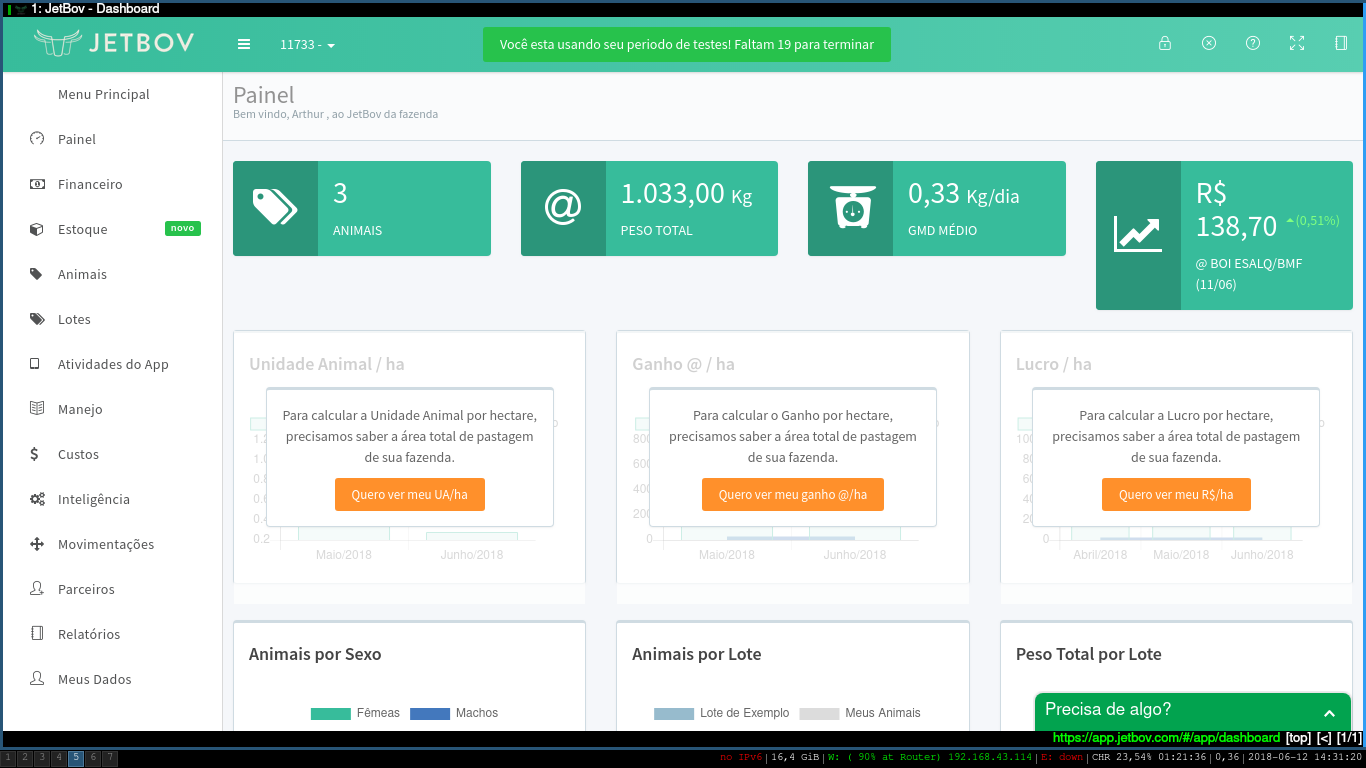
\includegraphics[width=6in]{img/jetbov.png}

		\floatfoot{Fonte: Autoria própria.}
	\end{center}
\end{figure}

%\begin{figure}[!h]
%\begin{center}
%\caption{Jetbov versão mobile - Página inicial}
%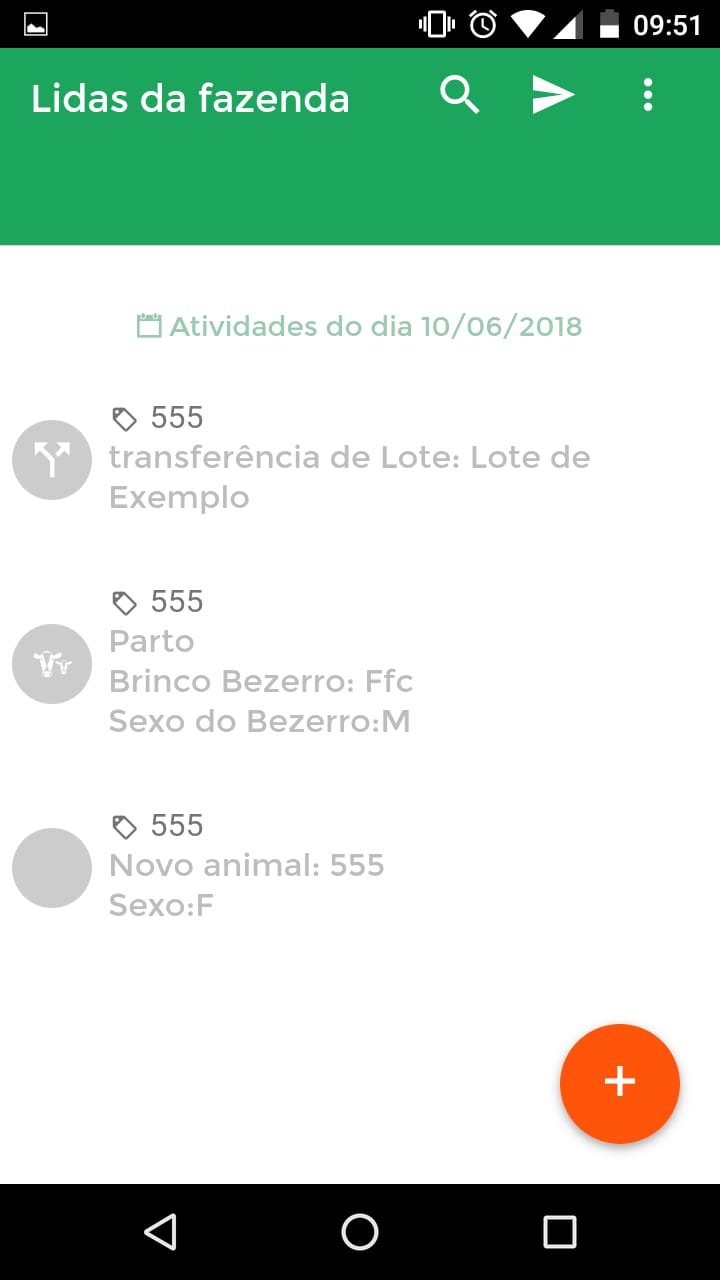
\includegraphics[width=6in]{img/jetbovapp1.jpeg}

%\floatfoot{Fonte: Autoria própria.}
%\end{center}
%\end{figure}

%\begin{figure}[!h]
%\begin{center}
%\caption{JetBov versão mobile - Opções de ações}
%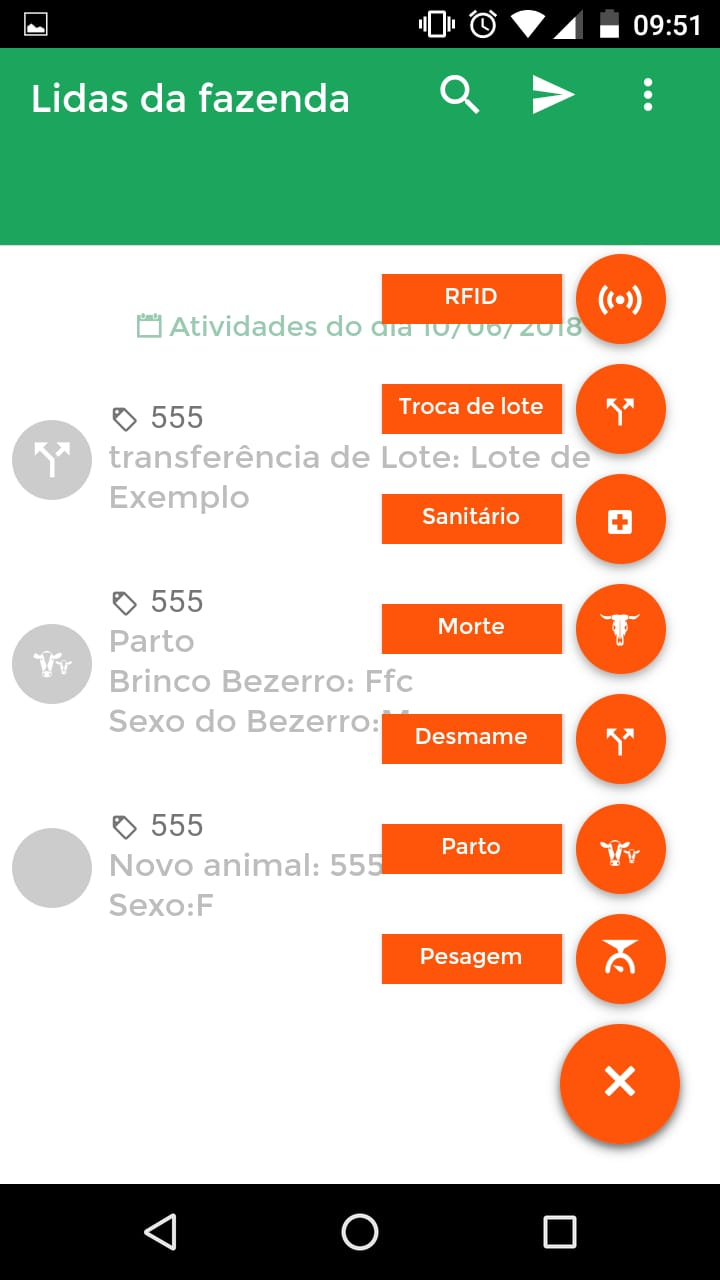
\includegraphics[width=6in]{img/jetbovapp2.jpeg}

%\floatfoot{Fonte: Autoria própria.}
%\end{center}
%\end{figure}

\newpage

\subsection{A3Pecuária}

A3Pecuária é um software para gestão de animais com controle de reprodução, pesagens, vacinas e exames, controle financeiro e de estoque e compra e venda. Segundo o site do fabricante: "fornecemos importantes informações de análise de seu rebanho de maneira simples e com uma interface muito fácil de aprender, permitindo gerir seu investimento de forma a aumentar a lucratividade" \cite{a3pecuaria16}.

Segundo \citeonline{a3pecuaria16}, são 3 tipos de planos, que variam de R\$ 29,90 a R\$ 69,90 por mês, e que gerenciam 500 animais ativos e 1 Fazenda até 3000 animais ativos e fazendas ilimitadas. Não possui versão gratuita, mas uma versão de testes por 30 dias.

Apresenta duas versões, uma web e outra mobile. A mobile, por ser simples, contém apenas a lista de animais da fazenda, o inventário, uma opção de bastão eletrônico e links para a versão web.

A versão web, por ser mais robusta e completa, apresenta uma série de possibilidades de manejos como novo lote, novo animal, nova despesa, nova receita e uma série de análise de dados com relatórios da propriedade.

A seguir, uma imagem mostrando a página inicial do sistema A3Pecuária versão web.

\newpage

\begin{figure}[!h]
	\begin{center}
		\caption{Página inicial da versão web do A3Pecuária}
		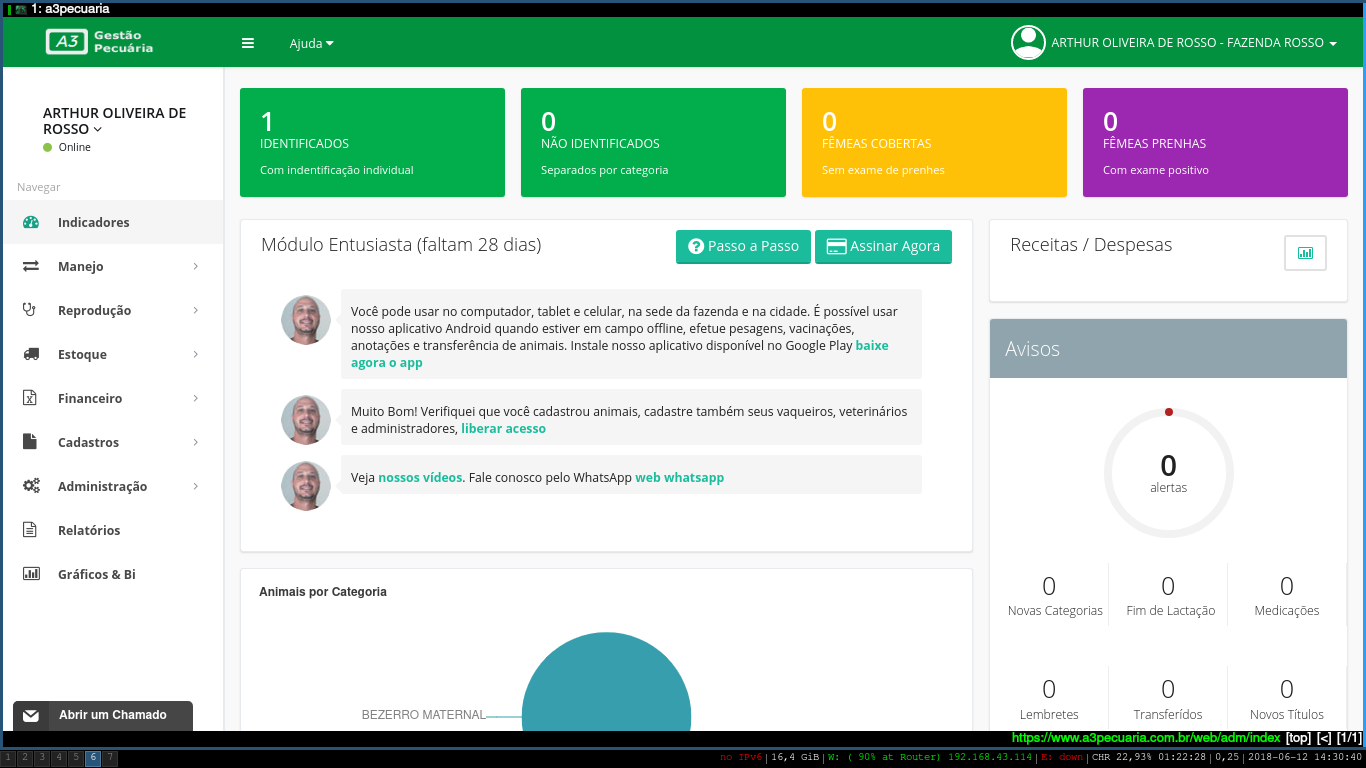
\includegraphics[width=6in]{img/a3pecuaria.png}

		\floatfoot{Fonte: Autoria própria.}
	\end{center}
\end{figure}

%\begin{figure}[!h]
%\begin{center}
%\caption{A3Pecuária versão mobile - Página inicial}
%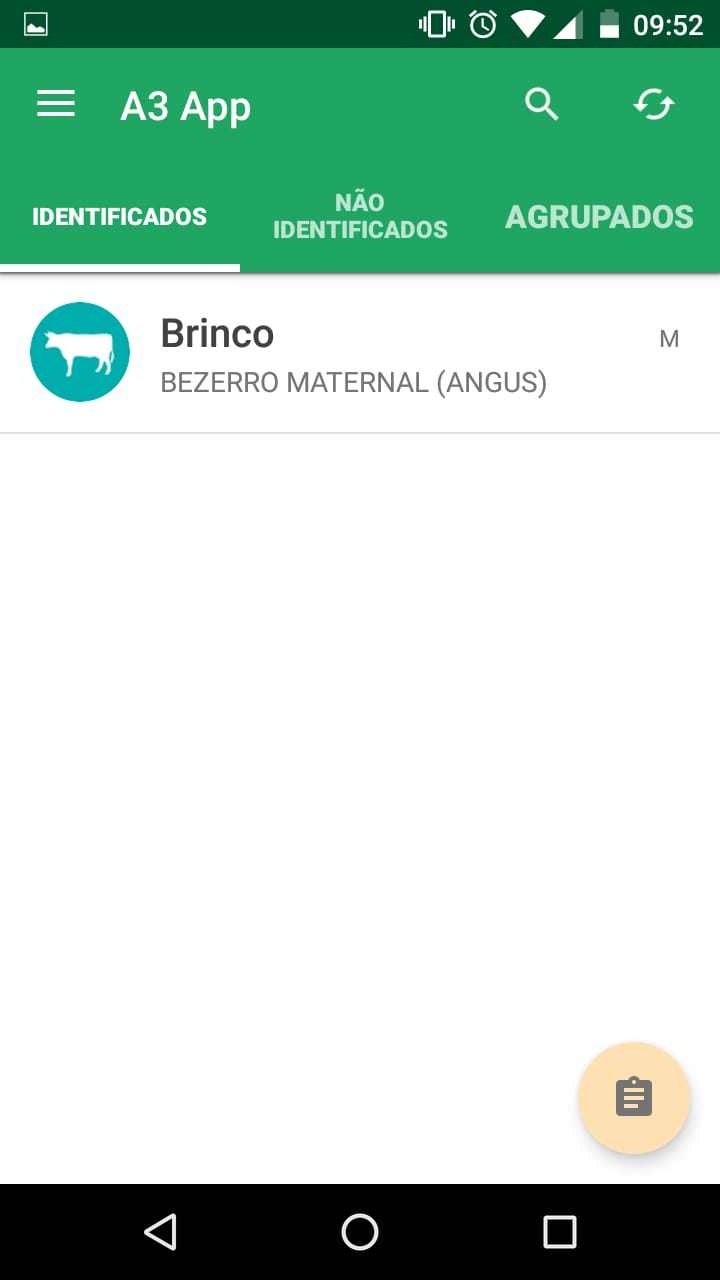
\includegraphics[width=6in]{img/a3pecuariaapp1.jpeg}

%\floatfoot{Fonte: Autoria própria.}
%\end{center}
%\end{figure}

%\begin{figure}[!h]
%\begin{center}
%\caption{A3Pecuária versão mobile - Opções de ações}
%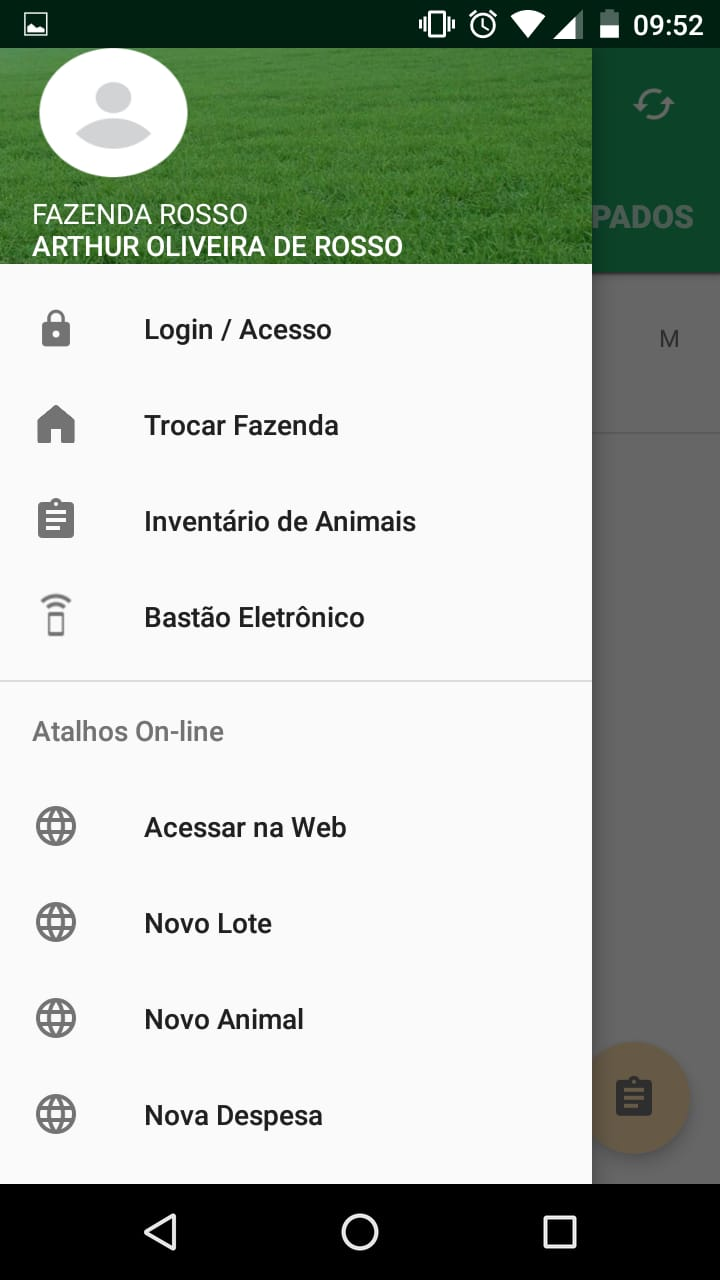
\includegraphics[width=6in]{img/a3pecuariaapp2.jpeg}

%\floatfoot{Fonte: Autoria própria.}
%\end{center}
%\end{figure}

\subsection{Análise Comparativa dos Trabalhos Relacionados}

Visto as análises de cada plataforma, podemos chegar na seguinte conclusão: todas tem seu modo de operação semelhante, como criar, deletar, ler e editar as informações de um animal, as opções de tratamento de gado (aqui chamado de manejo), as opções de estoques que no presente sistema é trabalhado só com medicações, e a visualização de relatórios são trabalhados de maneira parecida em todos os sistemas. Dessa maneira o presente sistema tem por objetivo trabalhar com estas mesmas operações, de maneira simples e sem custos.

\begin{center}
	\begin{tabular}{ | p{8cm} |  c | c | c | c |}
		\hline
		Funcionalidade & BovControl & JetBov & A3Pecuária & GoBov \\ \hline
		Gerenciamento de animais de uma propriedade & Sim & Sim & Sim & Sim \\  \hline
		Gerenciamento de medicamentos de uma propriedade & Não & Não & Sim & Sim  \\ \hline
		Gerenciamento de medicações de animais & Sim & Sim & Sim & Sim  \\ \hline
		Visualização de relatóris gerais da propriedade & Sim & Sim & Sim & Sim  \\ \hline
		Visualização de relatóris individuais de cada animal & Não & Não & Não & Sim  \\ \hline
		Versão gratuita & Sim & Não & Não & Sim  \\
		\hline
	\end{tabular}
\end{center}

\newpage

\section{Modelo de requisitos}

\subsection{Diagrama de Casos de uso}

O diagrama a seguir mostra os casos em que o sistema será utilizado, os casos de uso CD001 e CD002 já foram implementados e CD003 e CD004 estão em implementação conforme o cronograma.

\begin{figure}[!h]
	\begin{center}
		\caption{Diagrama de Casos de Uso do sistema}
		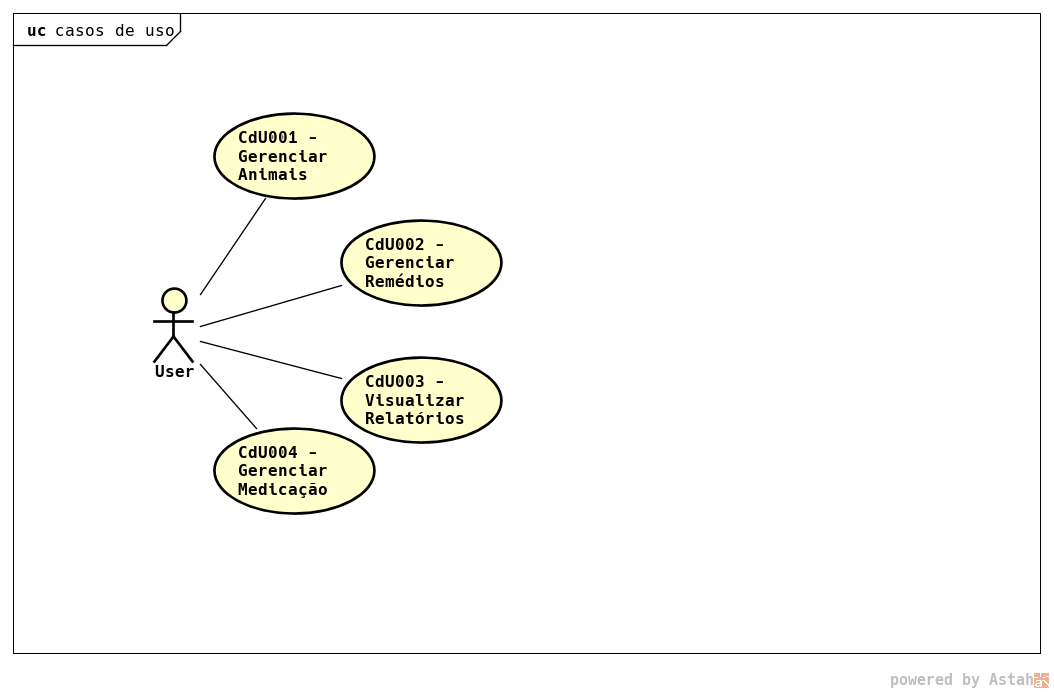
\includegraphics[width=6in]{img/casosdeuso.png}

		\floatfoot{Fonte: Autoria própria.}
	\end{center}
\end{figure}


\subsection{Especificação de Casos de Uso}

\begin{center}
	\begin{tabular}{ | l |  p{10cm} |}
		\hline
		Código e Nome do Caso de Uso & CdU001 - Gerenciar Animais \\ \hline
		Ator Primário: & Usuário \\ 
		Ator Secundário: & Não se aplica \\ \hline
		Fluxo Principal de Eventos & P1. O usuário solicita consultar os animais. \\
					   & P2. O sistema apresenta a tela de animais. (IV003) (A1) (A2) \\
					   & P3. O usuário solicita ver um animal em específico. \\
					   & P4. O sistema apresenta a tela de perfil do animal. (IV006) (A3) (A4)  \\
					   & P5. O caso de uso se encerra. \\ \hline
		Fluxo Alternativo:         & A1.1. Em P2 o usuário insere as informações de um animal no formulário e solicita salvá-las. \\
		A1. Adicionar animal       & A1.2. O sistema salva o animal. \\ 
					   & A1.3. Retorna ao P2. \\ \hline
		Fluxo Alternativo:         & A2.1. Em P2 o usuário tem a intenção de deletar um animal. \\
		A2. Deletar animal         & A2.2. O sistema apaga o animal selecionado. \\
					   & A2.3. Retorna ao P2. \\ \hline
		Fluxo Alternativo:         & A3.1. Em P4 o usuário decide editar animal. \\
		A3. Editar animal          & A3.2. O sistema apresenta a tela de editar animal. (IV007) \\
					   & A3.3. O usuário insere as novas informações do animal. \\
					   & A3.4. O sistema salva essas informações. \\
					   & A3.5. Retorna ao P4. \\ \hline
		Fluxo Alternativo:         & A4.1. Em P4 o decide adicionar uma nova pesagem do animal. \\
		A4. Adicionar peso         & A4.2. O sistema apresenta a tela de adicionar pesagem. (IV008) \\
					   & A4.3. O usuário insere as novas informações de peso do animal. \\
					   & A4.4. O sistema salva essas informações. \\
					   & A4.3. Retorna ao P4. \\ \hline
		Fluxo Alternativo:         & A5.1. Em P4 o usuário decide consultar detalhes do animal. \\
		A5. Consultar Detalhes     & A5.2. O sistema apresenta a tela de detalhes do animal. \\
					   & A5.3. Retorna ao P4. \\
		\hline
	\end{tabular}
\end{center}


\begin{center}
	\begin{tabular}{ | l |  p{10cm} |}
		\hline
		Código e Nome do Caso de Uso & CdU002 - Gerenciar Remédios \\ \hline
		Ator Primário: & Usuário \\ 
		Ator Secundário: & Não se aplica \\ \hline
		Fluxo Principal de Eventos & P1. O usuário solicita consultar os remédios. \\
					   & P2. O sistema apresenta a tela de remédios. (IV004) (A1) (A2) (A3) \\
					   & P3. O caso de uso se encerra. \\ \hline
		Fluxo Alternativo:         & A1.1. Em P2 o usuário insere as informações de um remédio no formulário e solicita salvá-las. \\
		A1. Adicionar remédio      & A1.2. O sistema salva o remédio. \\ 
					   & A1.3. Retorna ao P2. \\ \hline
		Fluxo Alternativo:         & A2.1. Em P2 o usuário resolve deletar um remédio. \\
		A2. Deletar remédio        & A2.2. O sistema apaga o remédio selecionado. \\
					   & A2.3. Retorna ao P2. \\ \hline
		Fluxo Alternativo:         & A3.1. Em P2 o usuário decide editar um remédio. \\
		A3. Editar remédio         & A3.2. O sistema apresenta a tela de editar remédio. \\
					   & A3.3. O usuário insere as novas informações do remédio. \\
					   & A3.4. O sistema salva essas informações. \\
					   & A3.5. Retorna ao P2. \\
		\hline
	\end{tabular}
\end{center}


\begin{center}
	\begin{tabular}{ | l |  p{10cm} |}
		\hline
		Código e Nome do Caso de Uso & CdU003 - Visualizar relatórios \\ \hline
		Ator Primário: & Usuário \\ 
		Ator Secundário: & Não se aplica \\ \hline
		Fluxo Principal de Eventos & P1. O usuário solicita consultar os relatórios. \\
					   & P2. O sistema apresenta a tela de relatórios da fazenda. \\
					   & P3. O caso de uso se encerra. \\
		\hline
	\end{tabular}
\end{center}



\begin{center}
	\begin{tabular}{ | l |  p{10cm} |}
		\hline
		Código e Nome do Caso de Uso & CdU004 - Gerenciar medicação \\ \hline
		Ator Primário: & Usuário \\ 
		Ator Secundário: & Não se aplica \\ \hline
		Fluxo Principal de Eventos & P1. O usuário solicita consultar medicação. \\
					   & P2. O sistema apresenta a tela de medicação. (IV005) (A1) (A2) (A3) \\
					   & P3. O caso de uso se encerra. \\ \hline
		Fluxo Alternativo:         & A1.1. Em P2 o usuário insere as informações de uma medicação e solicita salvá-las. \\
		A1. Adicionar medicação    & A1.2. O sistema salva a medicação. \\ 
					   & A1.3. Retorna ao P2. \\ \hline
		Fluxo Alternativo:         & A1.1. Em P2 o usuário resolve deletar uma medicação. \\
		A2. Deletar medicação      & A2.2. O sistema apaga a medicação selecionada. \\
					   & A2.3. Retorna ao P2. \\ \hline
		Fluxo Alternativo:         & A3.1. Em P2 o usuário decide editar uma medicação. \\
		A3. Editar medicação       & A3.2. O sistema apresenta a tela de editar medicação. \\
					   & A3.3. O usuário insere as novas informações da medicação. \\
					   & A3.4. O sistema salva essas informações. \\
					   & A3.5. Retorna ao P2. \\
		\hline
	\end{tabular}
\end{center}

\newpage

\subsection{Protótipos de Tela}

\subsubsection{IV001}

\begin{figure}[!h]
	\begin{center}
		\caption{Login no sistema}
		%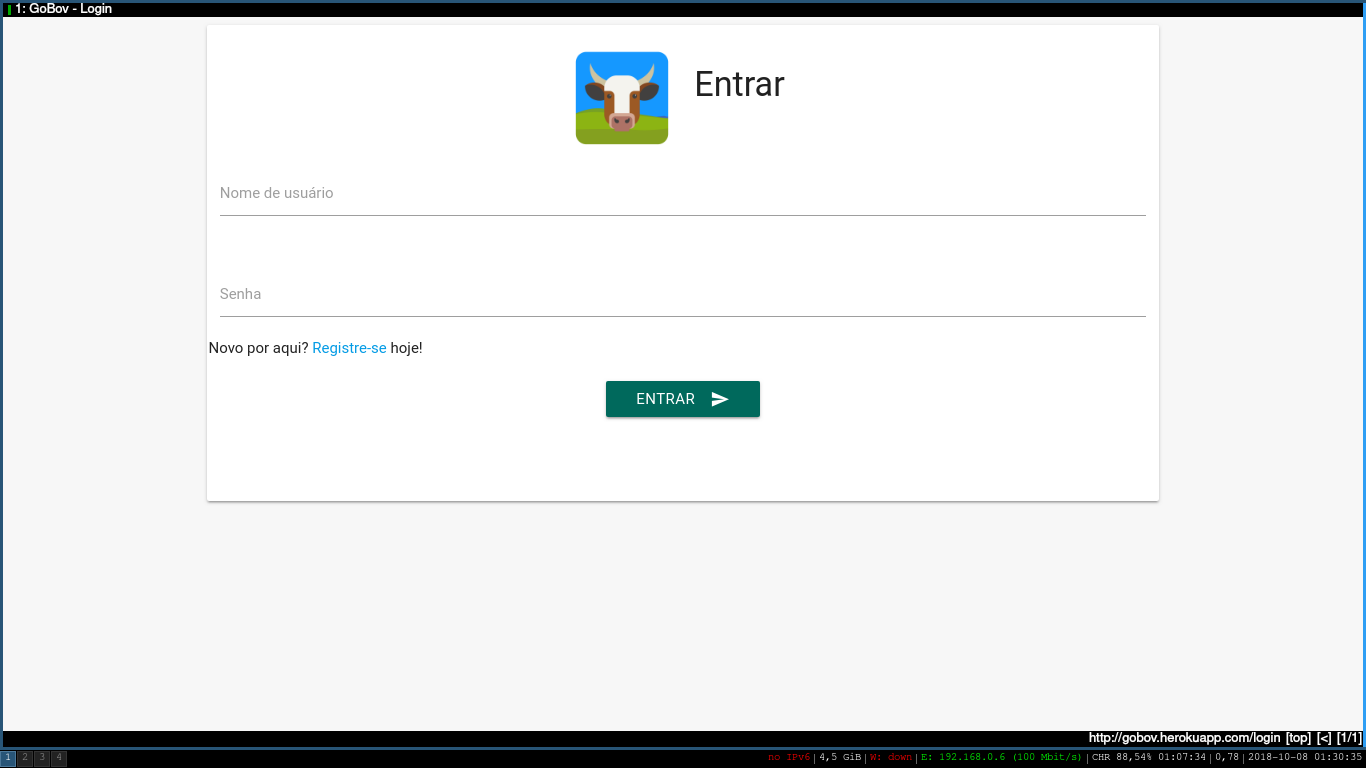
\includegraphics[width=13cm]{img/prototipos/login.png}

		%\floatfoot{Fonte: Autoria própria.}

	\end{center}
\end{figure}


\subsubsection{IV002}

\begin{figure}[!h]
	\begin{center}
		\caption{Página inicial do sistema}
		%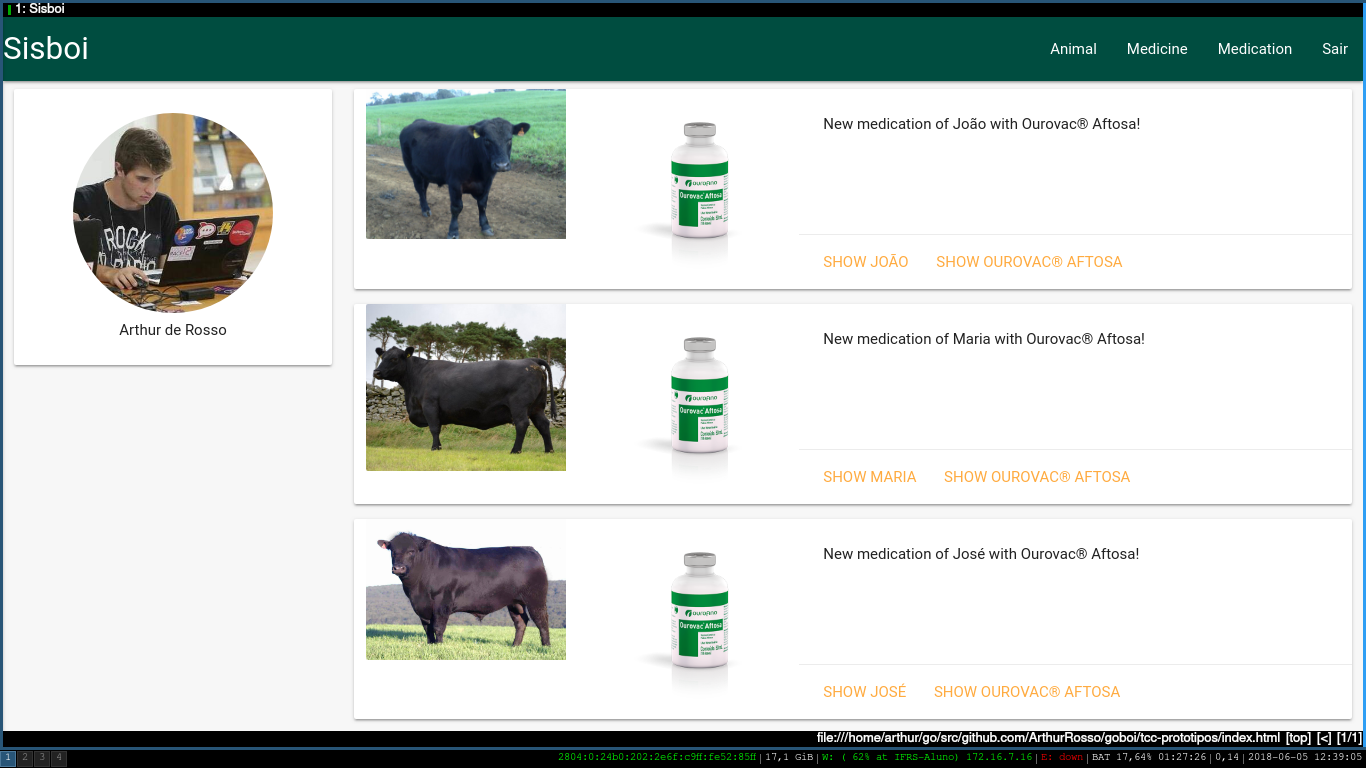
\includegraphics[width=13cm]{img/prototipos/index.png}

		%\floatfoot{Fonte: Autoria própria.}

	\end{center}
\end{figure}

\newpage

\subsubsection{IV003}

\begin{figure}[!h]
	\begin{center}
		\caption{Página do animal}
		%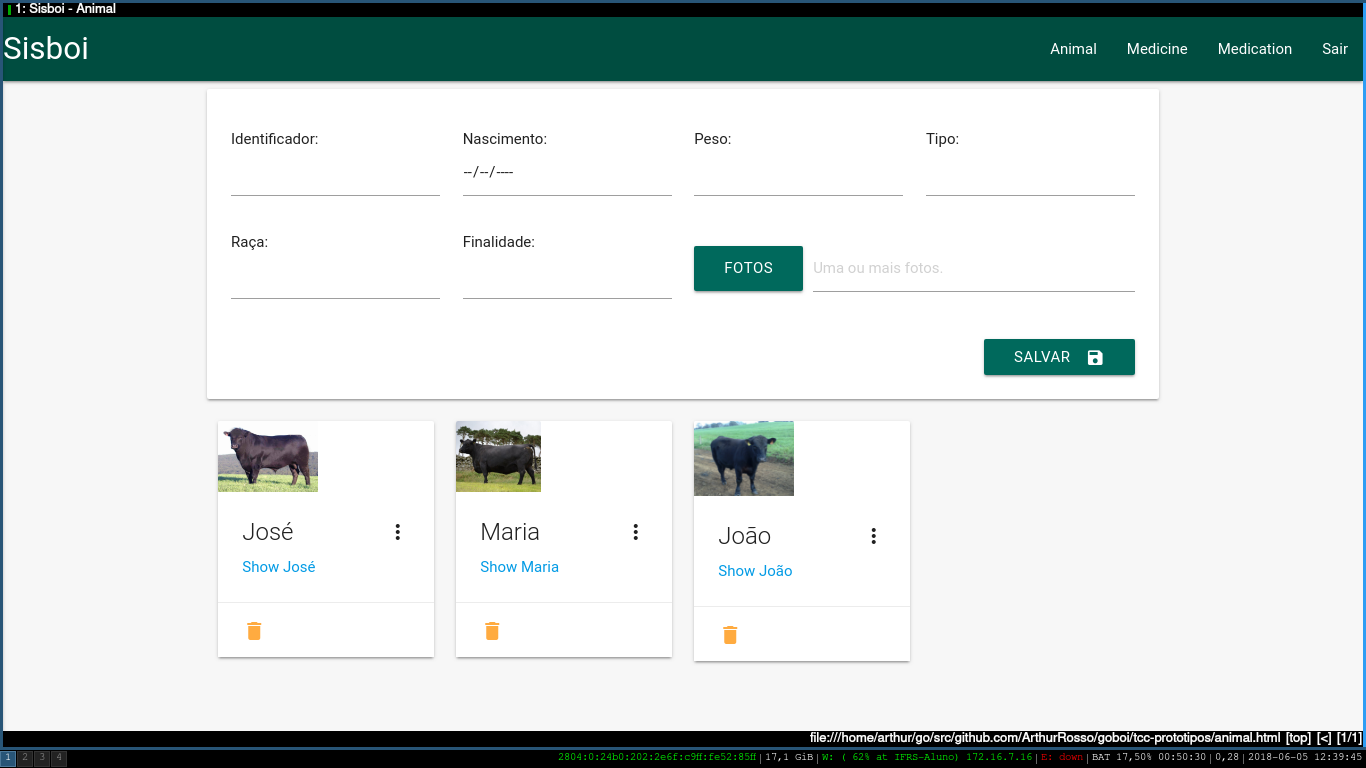
\includegraphics[width=13cm]{img/prototipos/animal.png}

		%\floatfoot{Fonte: Autoria própria.}

	\end{center}
\end{figure}


\subsubsection{IV004}

\begin{figure}[!h]
	\begin{center}
		\caption{Página de remédios}
		%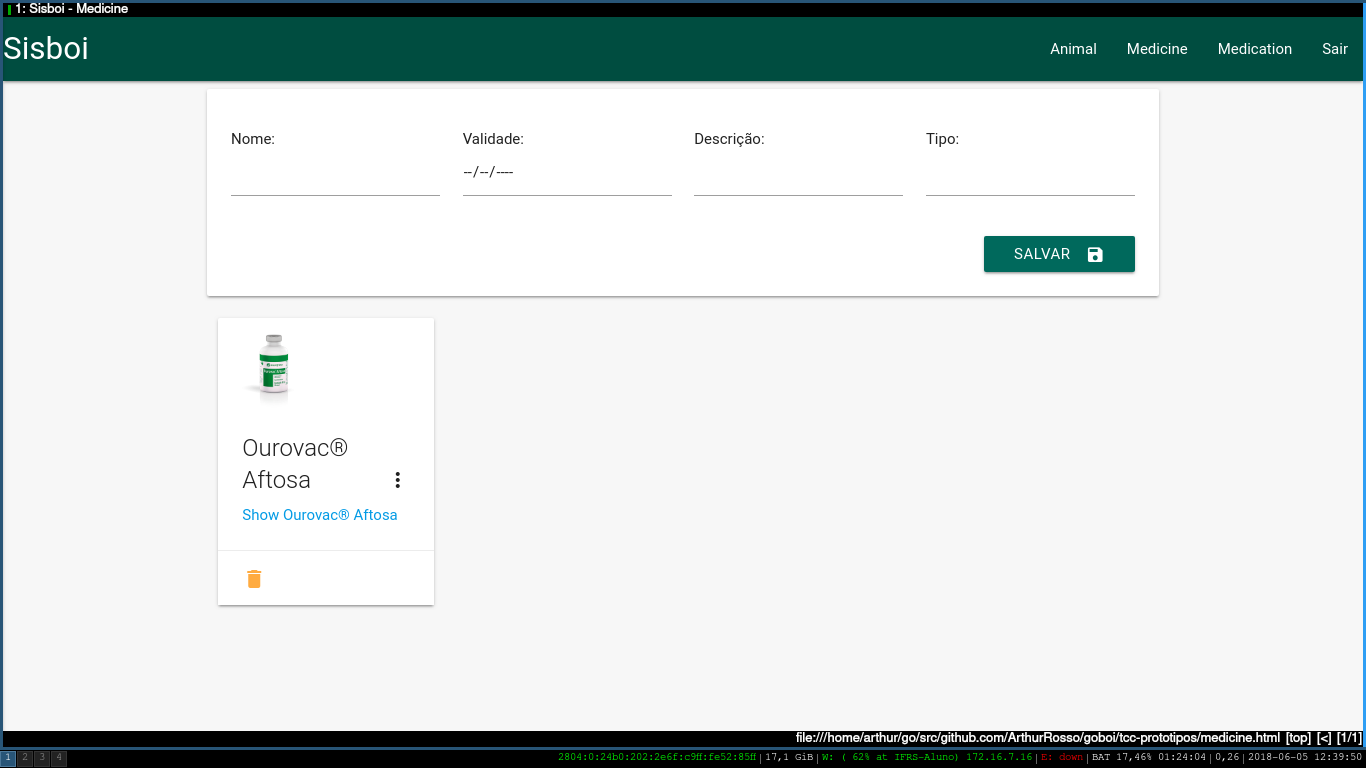
\includegraphics[width=13cm]{img/prototipos/remedio.png}

		%\floatfoot{Fonte: Autoria própria.}

	\end{center}
\end{figure}

\newpage

\subsubsection{IV005}

\begin{figure}[!h]
	\begin{center}
		\caption{Página de medicação}
		%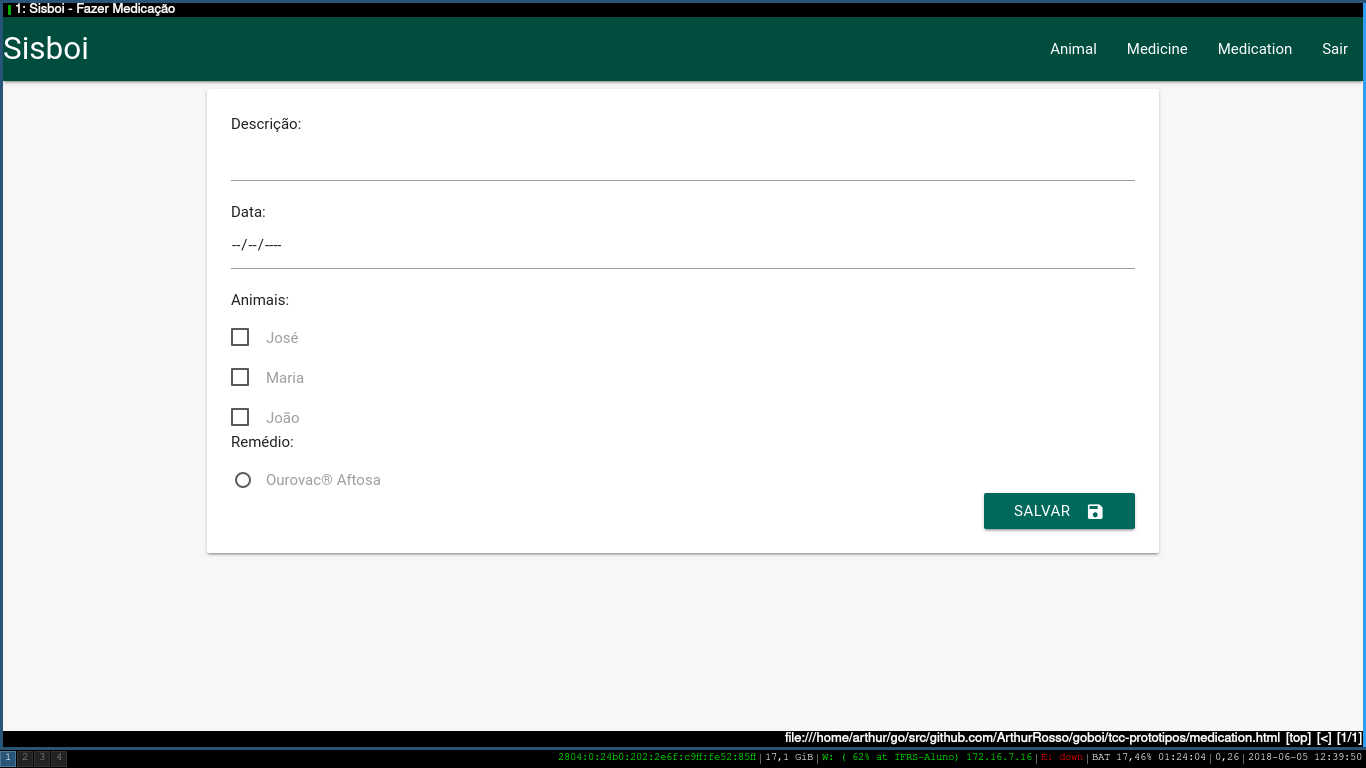
\includegraphics[width=13cm]{img/prototipos/medicacao.png}

		%\floatfoot{Fonte: Autoria própria.}

	\end{center}
\end{figure}


\subsubsection{IV006}

\begin{figure}[!h]
	\begin{center}
		\caption{Página de perfil do animal}
		%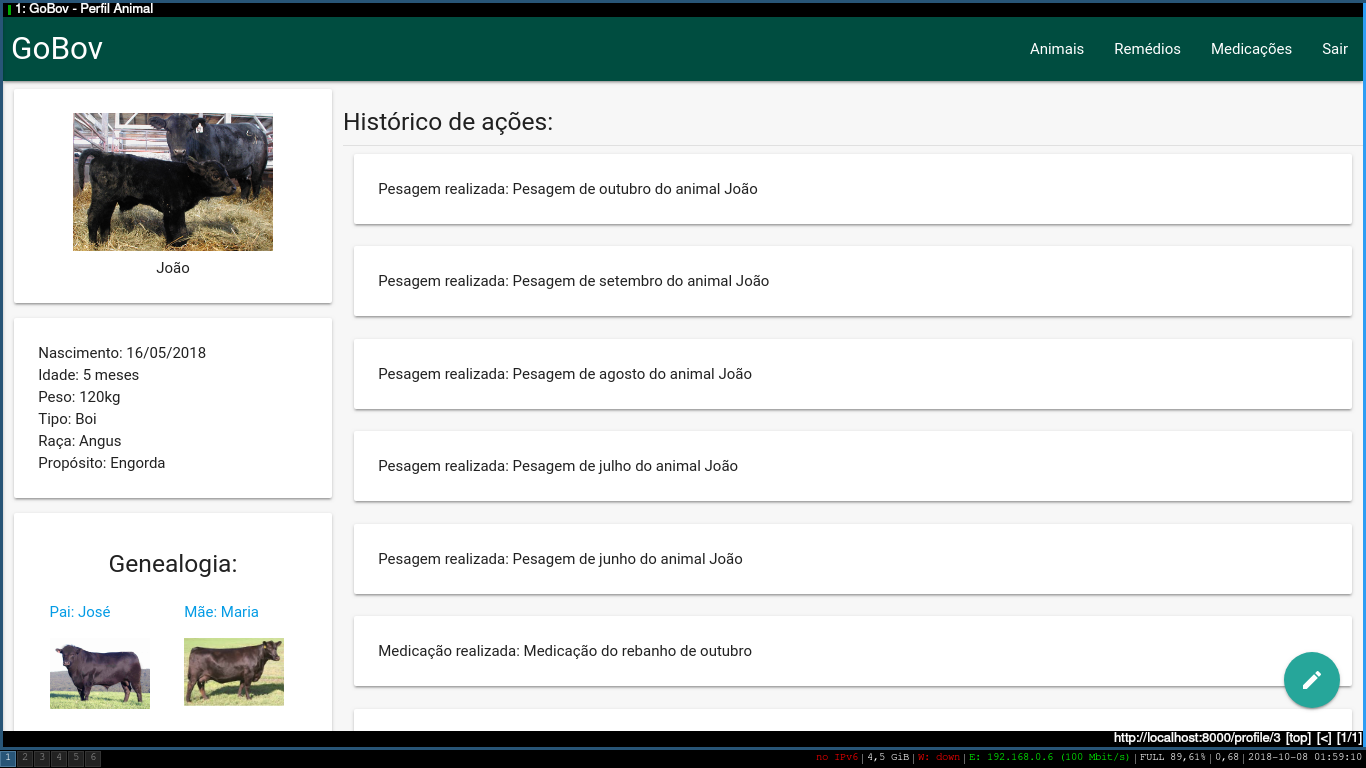
\includegraphics[width=13cm]{img/prototipos/perfil.png}

		%\floatfoot{Fonte: Autoria própria.}

	\end{center}
\end{figure}

\newpage

\subsubsection{IV007}

\begin{figure}[!h]
	\begin{center}
		\caption{Página de edição do animal}
		%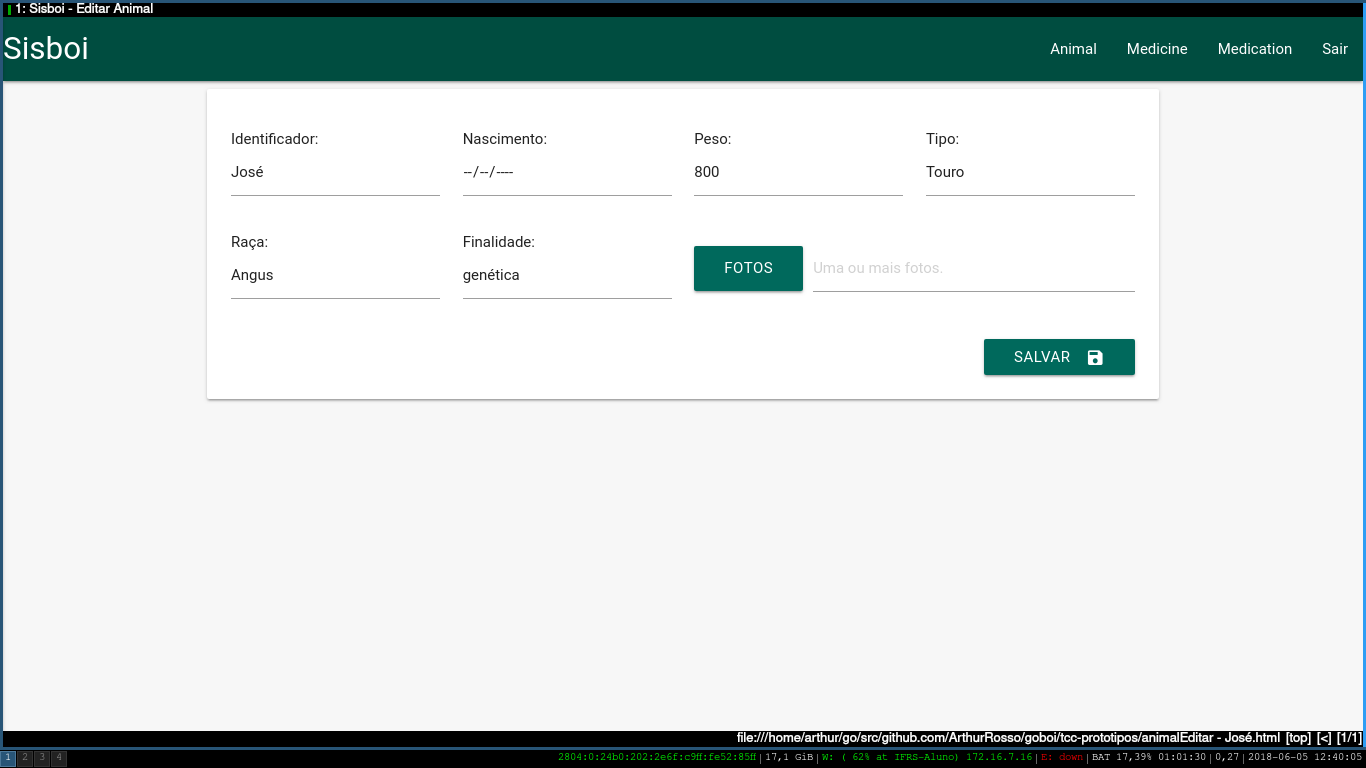
\includegraphics[width=13cm]{img/prototipos/editar.png}

		%\floatfoot{Fonte: Autoria própria.}

	\end{center}
\end{figure}


\subsubsection{IV008}

\begin{figure}[!h]
	\begin{center}
		\caption{Página de pesagem do animal}
		%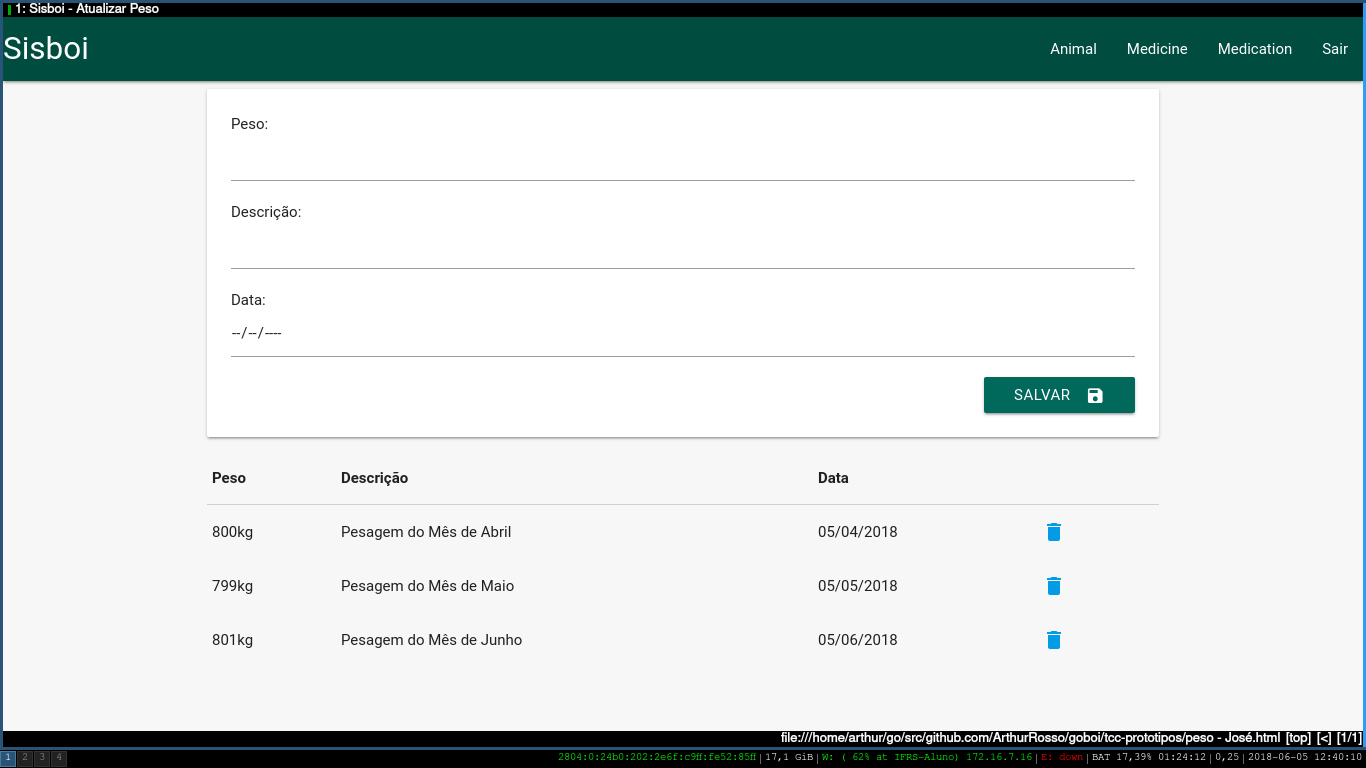
\includegraphics[width=13cm]{img/prototipos/peso.png}

		%\floatfoot{Fonte: Autoria própria.}

	\end{center}
\end{figure}


\newpage
\section{Modelagem do Sistema}

\subsection{Diagramas de Atividade}

O diagrama de atividade a seguir representa os passos para atingir os objetivos pertinentes ao gerenciamento do animal, é também o maior e mais complexo, pois possui a maior parte das interações com o sistema.

\begin{figure}[!h]
	\begin{center}
		\caption{Diagrama da Atividade de Gerenciar Animal}
		%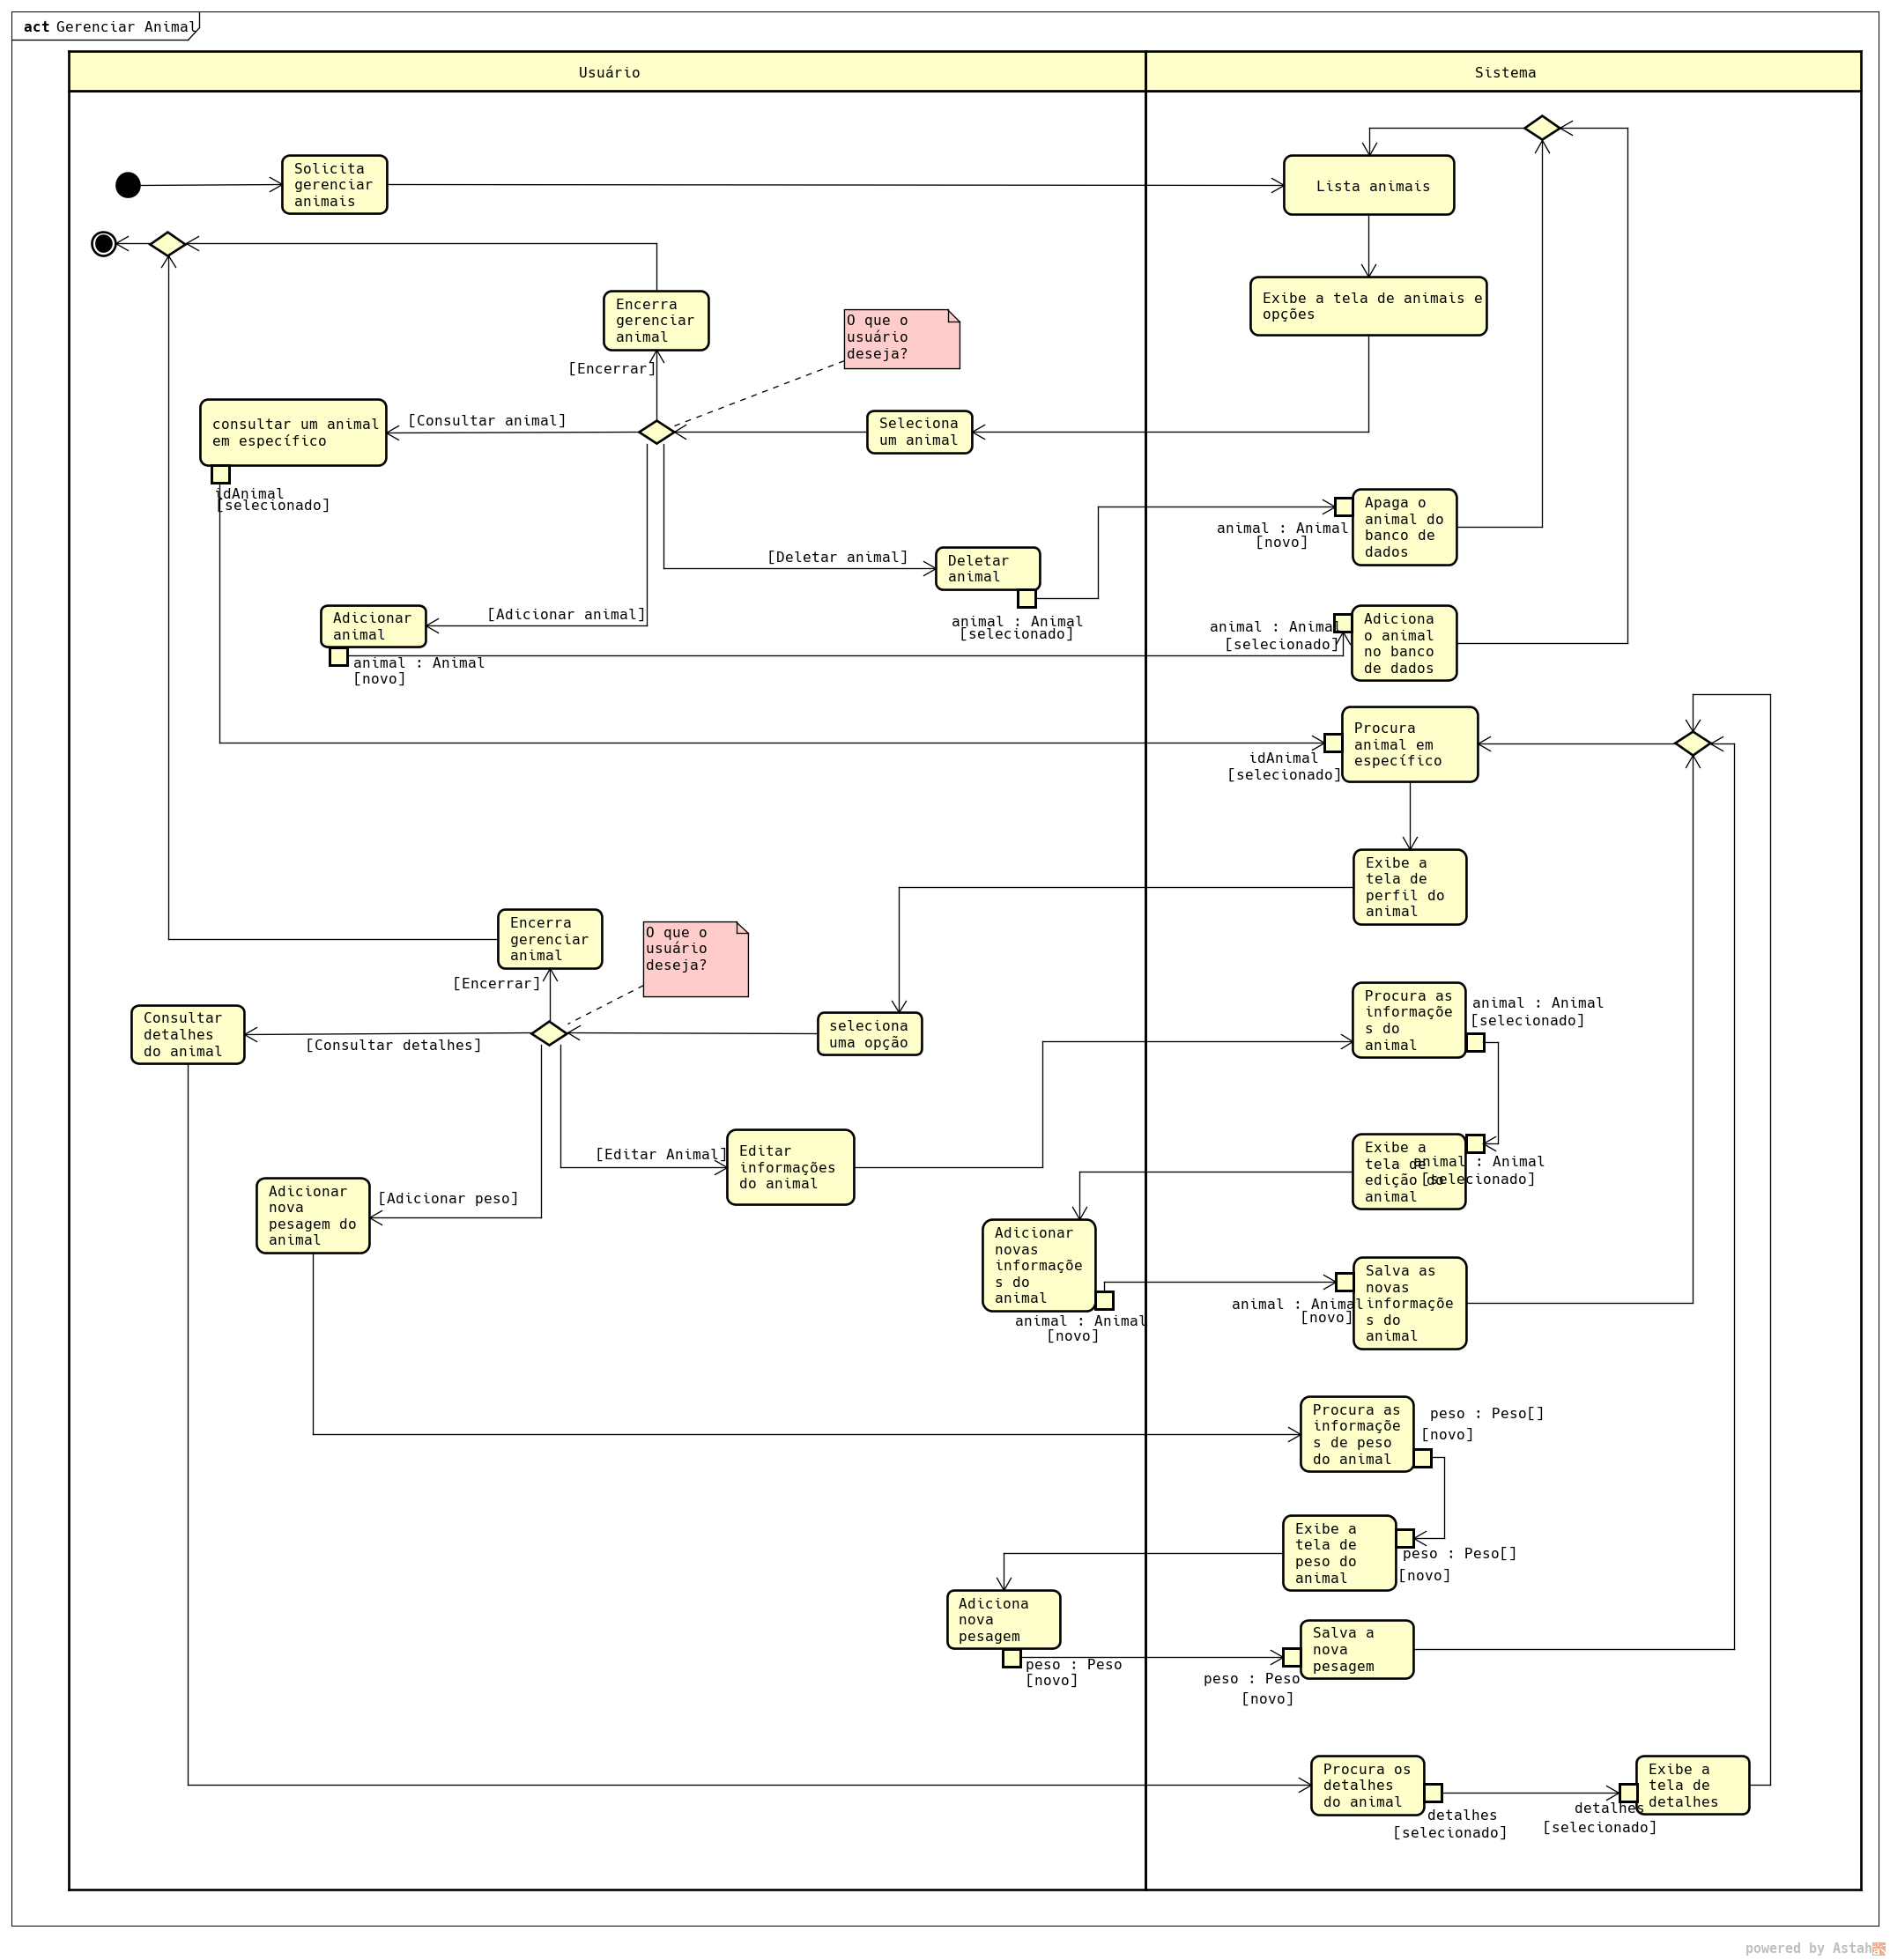
\includegraphics[width=6in]{img/atividadeanimal.png}

		%\floatfoot{Fonte: Autoria própria.}
	\end{center}
\end{figure}

\newpage

O diagrama a seguir descreve as interações do usuário com o sistema para gerenciar um remédio.

\begin{figure}[!h]
	\begin{center}
		\caption{Diagrama da Atividade de Gerenciar Remédios}
		%\includegraphics[width=6in]{img/atividaderememdio.png}

		%\floatfoot{Fonte: Autoria própria.}
	\end{center}
\end{figure}

\newpage

O diagrama a seguir descreve as interações do usuário com o sistema para gerenciar uma medicação.

\begin{figure}[!h]
	\begin{center}
		\caption{Diagrama da Atividade de Gerenciar Medicações}
		%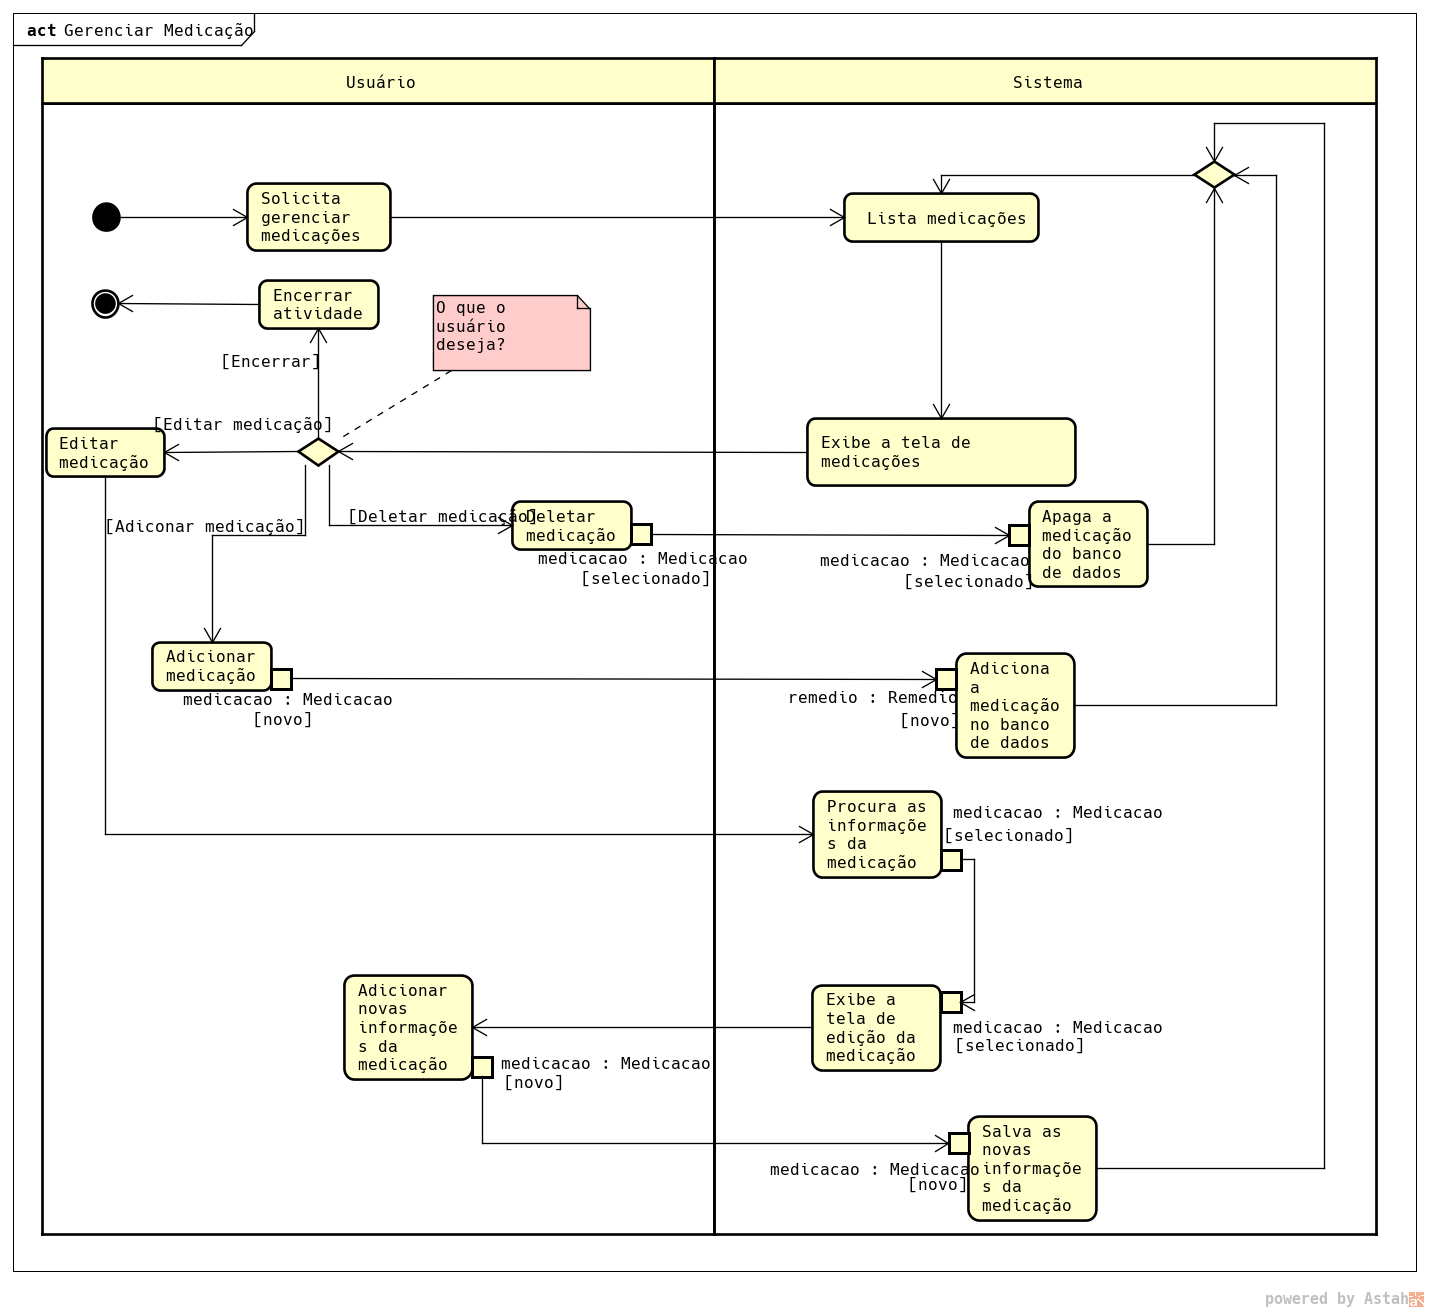
\includegraphics[width=6in]{img/atividademedicacao.png}

		%\floatfoot{Fonte: Autoria própria.}
	\end{center}
\end{figure}

\newpage

O diagrama a seguir mostra a atividade de visualizar os relatórios da propriedade rural.

\begin{figure}[!h]
	\begin{center}
		\caption{Diagrama da Atividade de Visualizar Relatórios}
		%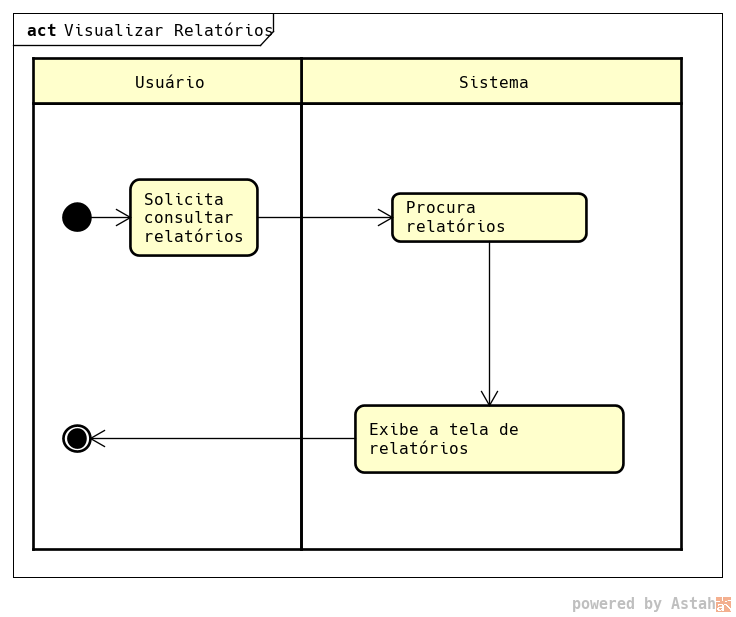
\includegraphics[width=6in]{img/atividaderelatorios.png}

		%\floatfoot{Fonte: Autoria própria.}
	\end{center}
\end{figure}

\newpage

\subsection{Modelagem do Banco de Dados}

O diagrama a seguir mostra a abstração do banco de dados representando a relação do animal com o usuário, com a foto, com o peso, com o propósito, com a raça, com o tipo, e com a remédio, na qual é chamada de medicação. Por sua vez, o remédio também tem uma relação além da medicação, que é o tipo.  

\begin{figure}[!h]
	\begin{center}
		\caption{Modelo ER}
		%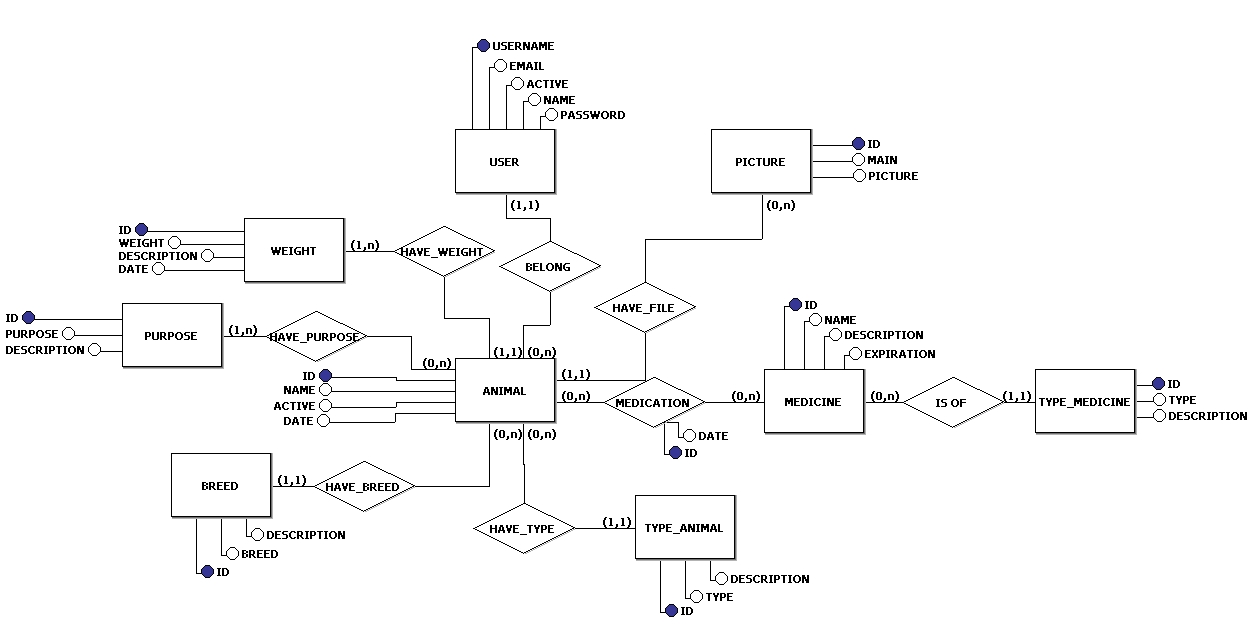
\includegraphics[width=6in]{img/erdoboi.jpeg}

		%\floatfoot{Fonte: Autoria própria.}

	\end{center}
\end{figure}

\newpage

\section{Proposta de Solução Tecnológica Escolhida}

\subsection{Metodologia}

\subsubsection{Metodologia de pesquisa}

Quanto a metodologia de pesquisa, optou-se pela abordagem qualitativa pois, "a pesquisa qualitativa não se preocupa com representatividade numérica, mas, sim, com o aprofundamento da compreensão de um grupo social, de uma organização, etc." \cite{ufrgs09}, dessa forma podemos nos aprofundar melhor e entender a realidade dos stakeholders. Possui natureza aplicada pois gerará conhecimentos destinados a solução de problemas específicos \cite{ufrgs09} .

Em relação ao procedimento foi adotado o estudo de caso,para \citeonline{yin01} este é uma investigação empírica que investiga um fenômeno contemporâneo dentro de seu contexto da vida real, especialmente quando os limites entre o fenômeno e o contexto não estão claramente definidos, esse foi o procedimento visto que o pesquisador analisou o caso de duas propriedades rurais localizadas no município de Caçapava do Sul e propôs uma solução de software para alguns dos problemas encontrados.

\subsubsection{Metodologia de desenvolvimento}

Quanto a metodologia de desenvolvimento, utilizou-se a UML (Unified Modeling Language) que, segundo \citeonline{fowler14} é uma família de notações gráficas, apoiadas por um metamodelo único, que ajuda na descrição e no projeto de sistemas de software, particularmente daqueles construídos utlizando o estilo orientado a objetos(OO).

Para tanto utilizou-se do diagrama de casos de uso porque, ele possibilita a compreensão do comportamento externo do sistema, tornando possível ter uma visão das funcionalidades do sistema \cite{guedes18}.

Também foi utilizado o diagrama de atividades, porque através dele é possível "descrever os passos a serem percorridos para a conclusão de uma atividade" \cite{guedes18}.

\subsection{Tecnologias Adotadas}

\begin{itemize}
	\item Golang: É uma linguagem de programação de código aberto que facilita a criação de software simples, confiável e eficiente. https://golang.org	
	\item MariaDB: É um banco de dados de código aberto bastante conhecido, é um fork do MySQL. https://mariadb.org/
	\item HTML: É uma linguagem de marcação de texto utilizada para desenvilver a estrutura de sites. https://www.w3.org/html/
	\item CSS: É uma linguagem  https://www.w3.org/Style/CSS/
	\item JavaScript: http://www.ecma-international.org/publications/standards/Stnindex.htm
	\item Materialize: https://materializecss.com/
\end{itemize}

\subsection{Ferramentas Adotadas}

\begin{itemize}
	\item Vim: https://www.vim.org
	\item phpMyAdmin: https://www.phpmyadmin.net
	\item BrModelo: http://www.sis4.com/brModelo/
	\item Astah: http://astah.net
	\item GORM: http://gorm.io
\end{itemize}

\newpage

\section{Cronograma}
\begin{table}[th]
	\resizebox{\textwidth}{!}{%
		\begin{tabular}{|c|c|c|c|c|c|c|c|c|c|c|c|c|}
			\hline
			\textbf{Atividade} & \textbf{Jan} & \textbf{Fev} & \textbf{Mar} & \textbf{Abr} & \textbf{Mai} & \textbf{Jun} & \textbf{Jul} & \textbf{Ago} & \textbf{Set} & \textbf{Out} & \textbf{Nov} & \textbf{Dez} \\ \hline
			\begin{tabular}[c]{@{}c@{}}Escolha\\ do Orientador\end{tabular}                  & X & & & & & & & & & & & \\ \hline
			\begin{tabular}[c]{@{}c@{}}Escolha\\ do Tema\end{tabular}                        & & X & & & & & & & & & & \\ \hline
			\begin{tabular}[c]{@{}c@{}}Apêndice I\end{tabular}                               & & & X & & & & & & & & & \\ \hline
			\begin{tabular}[c]{@{}c@{}}Apêndice II\end{tabular}                              & & & & X & X & & & & & & & \\ \hline
			\begin{tabular}[c]{@{}c@{}}Apêndice III\end{tabular}                             & & & & & X & X & & & & & & \\ \hline
			\begin{tabular}[c]{@{}c@{}}Elaboração do diagrama\\ de casos de uso\end{tabular} & & & & X & & & & & & & & \\ \hline
			\begin{tabular}[c]{@{}c@{}}Implementação do banco de dados\end{tabular}          & & & & X & & & & & & & & \\ \hline
			\begin{tabular}[c]{@{}c@{}}Implementar CRUD de animal\end{tabular}               & & & & X & X & & & & & & & \\ \hline
			\begin{tabular}[c]{@{}c@{}}Implementar CRUD de remédio\end{tabular}              & & & & & X & & & & & & & \\ \hline
			\begin{tabular}[c]{@{}c@{}}Implementar CRUD de medicação\end{tabular}            & & & & & & X & & & & & & \\ \hline
			\begin{tabular}[c]{@{}c@{}}Implementar painel de dados\end{tabular}              & & & & & X & X & & & & & & \\ \hline
			\begin{tabular}[c]{@{}c@{}}Apresentação Parcial\end{tabular}                     & & & & & & & X & & & & & \\ \hline
			\begin{tabular}[c]{@{}c@{}}Testes e Validações I\end{tabular}                    & & & & & & & & X & & & & \\ \hline
			\begin{tabular}[c]{@{}c@{}}Apresentação na IFCITEC\end{tabular}                  & & & & & & & & & X & & & \\ \hline
			\begin{tabular}[c]{@{}c@{}}Testes e Validações II\end{tabular}                   & & & & & & & & & & X & & \\ \hline
			\begin{tabular}[c]{@{}c@{}}Apresentação Final\end{tabular}                       & & & & & & & & & & & X & \\ \hline
		\end{tabular}%
	}
	\caption{Cronograma}
\end{table}

% \section{Conclusão}

% Deste modo, surgem alguns questionamentos: Qual a efetividade do sistema apresentado e quais os benefícios e contribuições para o usuário do sistema? Quais as consequências diante da inexistência do uso de registros do ciclo de vida animal? Tais questionamentos serão respondidos através do uso do sistema e da aplicação do mesmo.

\section{Referências}

\begingroup
\renewcommand{\section}[2]{}%
\bibliography{ApendiceIII}
\endgroup

\end{document}
